\documentclass{handout}

\SetInstructor{Lt Col James Phillips}
\SetCourseTitle{ECE231: Electrical Circuits and Systems I}
\SetSemester{Spring 2016}
\SetHandoutTitle{Lecture 20: Capacitors and Inductors}

%\SetDueDate{1 Jan 2016}
%\ShowAllBlanks

\showsoln \setsolncolor{red}

\begin{document}
\maketitle

\textbf{Upcoming events}
\begin{enumerate}
\item Problem Set \# 4 due Lesson 23
\item Homwork \# 5 due Lesson 25
\item Problem Set \# 5 due Lesson 25
\item Quiz \# 4 Lesson 26
\end{enumerate}

\textbf{OBJECTIVES:}
\begin{enumerate}
\item Understand $i$--$v$ characteristics for capacitors and inductors
\item Understand the capacitors and inductors can store energy
\item Be able to calculate equivalent capacitance and inductance
\end{enumerate}

\textbf{READING}
\begin{description}
\item [Required]:
\begin{itemize}
\item  Textbook, section 6.1, 6.2, 6.4, pages 281--293; 301--305
\end{itemize}
\item [Optional]: None
\end{description}

\textbf{HOMEWORK}
\begin{description}
\item [Required textbook problems]: 6.24, 6.44, 6.51, 6.55--- Due Lesson 23
\item [Recommended textbook problems]: None
\end{description}

\section{Capacitors}
A capacitor is a dynamic circuit element that can {\em store} or {\em dissipate} charge.  To start our discussion of capacitors, we will look at the cartoon of a parallel plate capacitor shown in Figure \ref{fig: Capacitor}

\begin{figure} [h!]
\centering
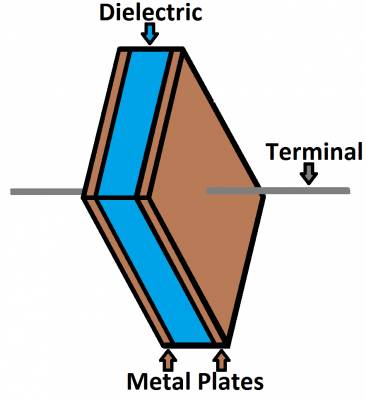
\includegraphics[width=0.3\textwidth]{Capacitor.jpg}
\caption{Parallel Plate Capacitor (borrowed from: learn.sparkfun.com)}
\label{fig: Capacitor}
\end{figure}

A parallel plate capacitor is just two metal plates (area, A) seperated by a distance, $d$.  If you accumulate a charge, $q$, on one plate, a negative charge, $-q$ accumulates on the other plate and an electric field exists between the two plates:

\soln{1in}{
\begin{equation}
\vec{\mathcal{E}}(t) = \frac{q(t)}{\epsilon A}
\end{equation}}
where $\vec{\mathcal{E}}(t)$ is the time varying E-field and $\epsilon$ is the permittivity of the dielectric.  This equation assume $d$ is small compared to $A$, but this is almost always a good assumption.  The units for the E-field are $\frac{V}{m}$ which implies the the E-field is related to a voltage, $v_c(t)$, between the plates:
\soln{0.6in}{
\begin{equation}
\vec{\mathcal{E}}(t) = \frac{v_c(t)}{d}
\end{equation}}
setting the last two equations equal to each other and solving for charge, $q(t)$ gives:
\soln{0.6in}{
\begin{equation}
q(t) = \left[\frac{\epsilon A}{d}  \right] v_c(t)
\end{equation}}

We will give that bracketed term a special name.  We will call it capacitance, $C$

\soln{0.6in}{
\begin{equation}
C = \frac{\epsilon A}{d}
\end{equation}}

which allows us to rewrite our charge equation

\soln{0.6in}{
\begin{equation}
q(t) = C v_c(t)
\end{equation}}

\subsection{$i$-$v$ Characteristic}
If we take the time derivative of our last equation we get:
\soln{0.6in}{
\begin{equation}
\frac{\partial q(t)}{\partial t} = C \frac{\partial v_c(t)}{\partial t}
\end{equation}}
but since $i_c(t) = \frac{\partial q(t)}{\partial t}$ we can rewrite this as
\soln{0.6in}{
\begin{equation}
i_c(t) = C \frac{\partial v_c(t)}{\partial t}
\end{equation}}
which gives us an $i$ - $v$ relationship for a capacitor.  I will leave this derivation to you, but you can write an integral form of this equation as:
\soln{0.6in}{
\begin{equation}
v_c(t) = v_c(0) +\frac{1}{C}\int_0^t i_c(x) dx
\end{equation}}
where $x$ is just a dummy variable for the integration.

\textbf{So what does this all mean?}

\soln{2in}{
\begin{enumerate}
\item A time varying voltage will create current through a capacitor
\item For DC voltage the current is zero (Open Circuit)
\item Capacitor voltage is a continuous function of time
\end{enumerate}
}

\newpage
\clearpage
\pagebreak

\textbf{Example 1 --Textbook Exercise 6-1} A $1\ \mu F$ capacitor has no voltage across it at $t=0$.  A current flowing through the capacitor is give as:
\begin{equation}
i_c(t) = 2u(t)-3u(t-2)+u(t-4)\ \mu A
\end{equation}
Find $v_c(t)$ at $t=4\ s$

\soln{3in}{
\begin{figure} [h!]
\centering
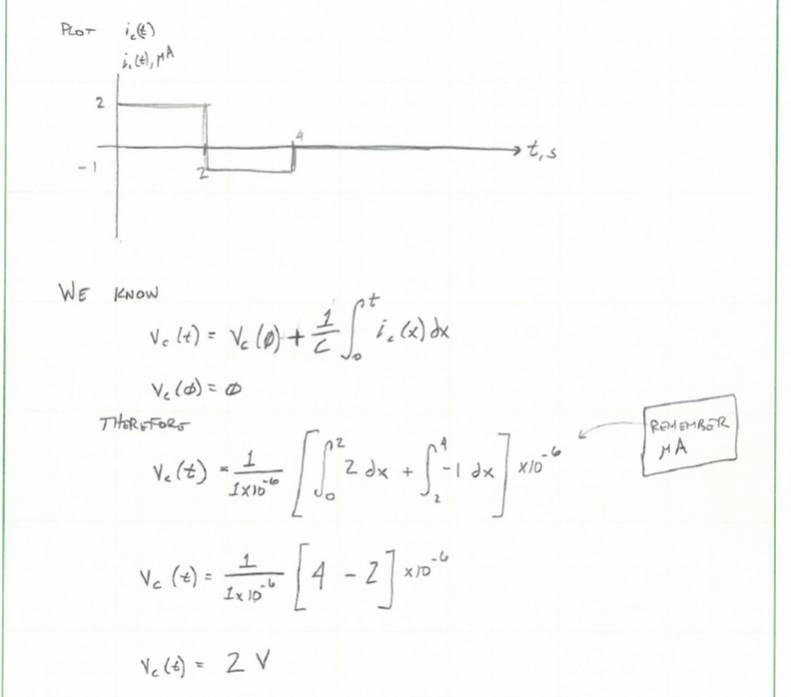
\includegraphics[width=1\textwidth]{Example1.jpg}
\end{figure}
}

\newpage
\clearpage
\pagebreak

\subsection{Power and Energy}
Power for a capacitor is found using the power law
\soln{1in}{
\begin{equation}
p_c(t) = v_c(t)i_c(t)
\end{equation}}
but using what we learned above, we can write this as
\soln{1in}{
\begin{equation}
p_c(t) = Cv_c(t)\frac{\partial v_c(t)}{\partial t}
\end{equation}}
which can also be written as (using the product rule):
\soln{1in}{
\begin{equation}
p_c(t) = \frac{\partial}{\partial t}\left[\frac{1}{2}Cv_c^2(t)\right]
\end{equation}}

Notice that the voltage across the capacitor and the time rate of change of the voltage can have like or opposite signs.  For example: $v_c = 5\ V$ and is decreasing would give opposite signs, while $v_c = 5\ V$ and is increasing would be like signs.

\textbf{Why is this important?} -- 

\soln{2in}{
Recall the power law.... A negative result in a power calculation tells us that the device is providing power while a positive result tells us a device is consuming power.  Capacitor power can be positive or negative... This means CAPACITORS CAN BOTH BE SOURCES AND SINKS FOR POWER.....  A capacitor can store energy!
}

\newpage
\clearpage
\pagebreak

\textbf{Example 2 -- Textbook Exercise 6-2(a) and 6-4 (a)} --- The voltage across a $10\ \mu F$ capacitor is 
\begin{equation}
v_c(t) = 25\sin(2000t)u(t)\ V
\end{equation}

Derive an expression for the current, $i_c(t)$ through the capacitor.  

Also find the power for the capacitor.  

Is the capacitor absorbing or delivering power at $t = 1\ s$?

\soln{4in}{
Current Expression:
\begin{equation}
i_c(t) = C \frac{\partial v_c(t)}{\partial t}
\end{equation}
\begin{equation}
i_c(t) = 25 \times 10\ \mu F \frac{\partial}{\partial t}\left[\sin(2000t)u(t)\right]
\end{equation}
\begin{equation}
i_c(t) = 500 \cos(2000t)u(t)\ mA
\end{equation}

Power:
\begin{equation}
p_c(t) = v_c(t)i_c(t)
\end{equation}
\begin{equation}
p_c(t) = \left[25\sin(2000t)u(t)\ V\right] \times \left[ 500 \cos(2000t)u(t)\ mA \right]
\end{equation}
\begin{equation}
p_c(t) = 12.5 \sin (2000t) \cos(2000t) u(t) \ W
\end{equation}
\begin{equation}
p_c(t) = 6.25 \sin (4000t)u(t) \ W
\end{equation}
This step relied on this trig identity $\sin(2\theta) = 2\sin(\theta)\cos(\theta)$
At $t=1\ s$:
\begin{equation}
p_c(1) = 6.25 \sin (4000) \ W = -4.27\ W
\end{equation}
Therefore the capcitor is delivering power!
}

\newpage
\clearpage
\pagebreak

\section{Inductors}
Our next {\em dynamic} circuit element to discuss is the inductor.  The inductor relies on the fact that when current flows in a wire, a magnetic field is induced around that wire (it follows the right hand rule!).  If we were to coil the wire, the magnetic flux would concentrate along the axis of the coil; see Figure \ref{fig: Inductor}. The magnetic flux wil be proportional to the current and the number of turns of wire:
\soln{1in}{
\begin{equation}
\phi(t) = \frac{\mu N A}{l}i_L(t)
\end{equation}
where $\mu$ is the permeability of the core, $l$ is the length of the coil, ans $A$ is the cross sectional area.
}

\begin{figure} [h!]
\centering
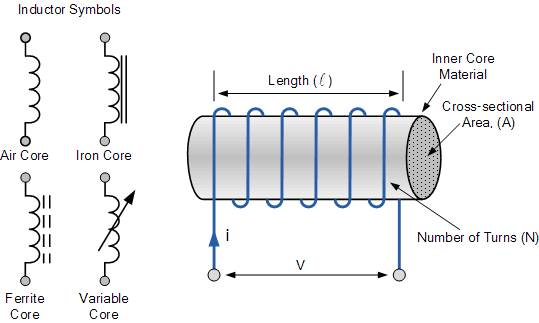
\includegraphics[width=0.6\textwidth]{Inductor.jpg}
\caption{A basic inductor (borrowed from: http://www.electronics-tutorials.ws)}
\label{fig: Inductor}
\end{figure}

We will say that the magnetic flux along the axis of this coil of wire links the turns of the coil and we will define the flux linkage, $\lambda$, by
\soln{1in}{
\begin{equation}
\lambda(t) = N\phi(t)
\end{equation}
}

We can combine the last 2 equations to get
\soln{1in}{
\begin{equation}
\lambda(t) = \frac{\mu N^2 A}{l}i_L(t)
\end{equation}
}

We will now give the proportionality constant above a special name, inductance, and give it the symbol, $L$:
\soln{1in}{
\begin{equation}
L= \frac{\mu N^2 A}{l}
\end{equation}
}
which gives
\soln{1in}{
\begin{equation}
\lambda(t) = Li_L(t)
\end{equation}
}

\newpage
\clearpage
\pagebreak


\subsection{Inductor $i$-$v$ Characteristic}
On the first day of class we offered the following definition of voltage:
\soln{1in}{
\begin{equation}
v(t) = \frac{\partial \lambda}{\partial t}
\end{equation}
}

Combining this with the last equation gives us:
\soln{1in}{
\begin{equation}
v_L(t) = L\frac{\partial }{\partial t}i_L(t)
\end{equation}
}

which is the $i$--$v$ relationship for an inductor. We can also write this integral form:
\soln{1in}{
\begin{equation}
i_L(t) =i_L(0)+ \frac{1}{L}\int_0^t v_L(x)dx
\end{equation}
}

\textbf{So what does this all mean?}

\soln{2in}{
\begin{enumerate}
\item A time varying current will create voltage across an inductor
\item For DC current the voltage is zero (Short Circuit)
\item Inductor current is a continuous function of time
\end{enumerate}
}

\newpage
\clearpage
\pagebreak

\subsection{Power and Energy}
Inductor power can be written as:
\soln{1in}{
\begin{equation}
p_L(t) = v_L(t)i_L(t)
\end{equation}}

which using our $i$--$v$ characteristic, we can rewrite as
\soln{1in}{
\begin{equation}
p_L(t) = Li_L(t)\frac{\partial }{\partial t}i_L(t)=\frac{1}{2}L\frac{\partial}{\partial t}i_L^2(t)
\end{equation}}


The current through the inductor $i_L(t)$ and its time derivative can have like or opposite signs; this means (like a capacitor) that an inductor can be a power source or power sink.  When an inductor is {\em sinking} power, it is storing energy that will be delivered back to the circuit at a later time.

\textbf{Example 3 -- Textbook Excercise 6-6}--- For $t>0$, the voltage across the a $4\ mH$ inductor is $v_L(t) = 20e^{-2000t}$ \& $i_L(0) = 0$.  

Find:\\
(a) The current through the inductor for $t>0$ \\
(b) The power for $t>0$?

\soln{4in}{
Current:
\begin{eqnarray}
i_L(t) &=&i_L(0)+ \frac{1}{L}\int_0^t v_L(x)dx \nonumber \\
i_L(t) &=&\frac{1}{4\times 10^{-3}}\int_0^t 20e^{-2000x}dx \nonumber \\
i_L(t) &=&-\frac{1}{2000 \times 4\times 10^{-3}}\left[20e^{-2000x}\right]_0^t  \nonumber \\
i_L(t) &=&2.5\left[1-e^{-2000t} \right] \ A \nonumber
\end{eqnarray} 
Power:
\begin{eqnarray}
p_L(t) &=& Li_L(t)\frac{\partial }{\partial t}i_L(t)\nonumber \\
p_L(t) &=& 4\times10^{-3}\times2.5\left[1-e^{-2000t} \right]\frac{\partial }{\partial t}2.5\left[1-e^{-2000t} \right]\nonumber \\
p_L(t) &=& 25\times 10^{-3}\left[1-e^{-2000t} \right]\left[2000e^{-2000t} \right]\nonumber \\
p_L(t) &=& 50\left[e^{-2000t}-e^{-4000t} \right]\ W \nonumber
\end{eqnarray} 
}

\newpage
\clearpage
\pagebreak

\textbf{Example 4-- Textbook Exercise 6-7}--- For $t<0$ current through a $100\ mH$ inductor is zero.  For $t\ge 0$, the current is $i_L(t) = 20e^{-2000t}-20e^{-4000t}\ mA$

(a) Derive an expression for the inductor voltage\\
(b) Find the time where the votage passes through zero\\
(c) Derive an expression for inductor power\\
(d) Find time intervals for when the inductor absorbs or delivers power\\

\soln{6in}{
Voltage:
\begin{eqnarray}
v_L(t) &=& L\frac{\partial }{\partial t}i_L(t) \nonumber \\
v_L(t) &=& 100\times 10^{-3}\frac{\partial }{\partial t} \left[20e^{-2000t}-20e^{-4000t}\right] \nonumber \\
v_L(t) &=& 2000\times 10^{-3} \left[-2000e^{-2000t}+4000e^{-4000t}\right] \nonumber \\
v_L(t) &=& 4000 \left[2e^{-4000t}-e^{-2000t}\right] \ mV  \nonumber \\
v_L(t) &=& 4 \left[2e^{-4000t}-e^{-2000t}\right] \ V  \nonumber
\end{eqnarray} 

Where does $v_L(t) =0$?
\begin{eqnarray}
2e^{-4000t}-e^{-2000t} &=& 0  \nonumber \\
2e^{-4000t} &=& e^{-2000t}  \nonumber \\
\ln 2e^{-4000t} &=& \ln e^{-2000t}  \nonumber \\
\ln 2 + \ln e^{-4000t} &=& \ln e^{-2000t}  \nonumber \\
0.693 &=& 2000t  \nonumber \\
t &=& 0.347\ ms \nonumber
\end{eqnarray} 

Inductor Power:
\begin{eqnarray}
p_L(t) &=& v_L(t)i_L(t) \nonumber \\
p_L(t) &=& 4 \left[2e^{-4000t}-e^{-2000t}\right]\times 20 \times 10^{-3}\left[e^{-2000t}-e^{-4000t}\right]\nonumber \\
p_L(t) &=& 80\times 10^{-3} \left[3e^{-6000t}-2e^{-8000t}-e^{-4000t}\right]  \nonumber \\
p_L(t) &=& -80e^{-4000t}+240e^{-6000t}-160e^{-8000t} \ mW \nonumber
\end{eqnarray} 

Absorbing or delivering?

We know from part (b) that hte zero crossing is at $t=0.347\ ms$.  Lets check the sign of our power at a point above and below that cut off.
\begin{eqnarray}
p_L(0.1\ ms) &=& -80e^{-4000 \times 0.0001}+240e^{-6000 \times 0.0001}-160e^{-8000 \times 0.0001} \ mW \nonumber\\
p_L(0.1\ ms) &=&6.19 \ mW
\end{eqnarray} 
\begin{eqnarray}
p_L(0.5\ ms) &=& -80e^{-4000 \times 0.0005}+240e^{-6000 \times 0.0005}-160e^{-8000 \times 0.0005} \ mW \nonumber\\
p_L(0.5\ ms) &=&-1.81 \ mW
\end{eqnarray} 

Therefore (based on the passive sign convention) power is absorbed for $t<0.347\ ms$ and delivered for $t>0.347\ ms$
}


\newpage
\clearpage
\pagebreak

\section{Equivalent Capacitance and Inductance}
I am going to give you the equations without a derivation or proof.  Please see the book for derivation.

\subsection{Equivalent Capacitance}
\textbf{Parallel Connection}
\soln{1in}{
\begin{equation}
C_{eq} = \sum_{n=1}^k C_n
\end{equation}
}

\textbf{Series Connection}
\soln{1in}{
\begin{equation}
C_{eq} = \left[\sum_{n=1}^k \frac{1}{C_n}\right]^{-1}
\end{equation}
}

\subsection{Equivalent Inductance}

\textbf{Parallel Connection}
\soln{1in}{
\begin{equation}
L_{eq} = \left[\sum_{n=1}^k \frac{1}{L_n}\right]^{-1}
\end{equation}
}

\textbf{Series Connection}
\soln{1in}{
\begin{equation}
L_{eq} = \sum_{n=1}^k L_n
\end{equation}
}

\newpage
\clearpage
\pagebreak

\section{Practical Circuits}
Over the last few lessons, we have learned about Op Amps, Capacitors and Inductors.  Can we build any practical curcuits using these devices?  Let's begin by looking at the circuit in Figure \ref{fig: Integrator}.  Let's analyze this circuit to determine what it does.

\begin{figure} [h!]
\centering
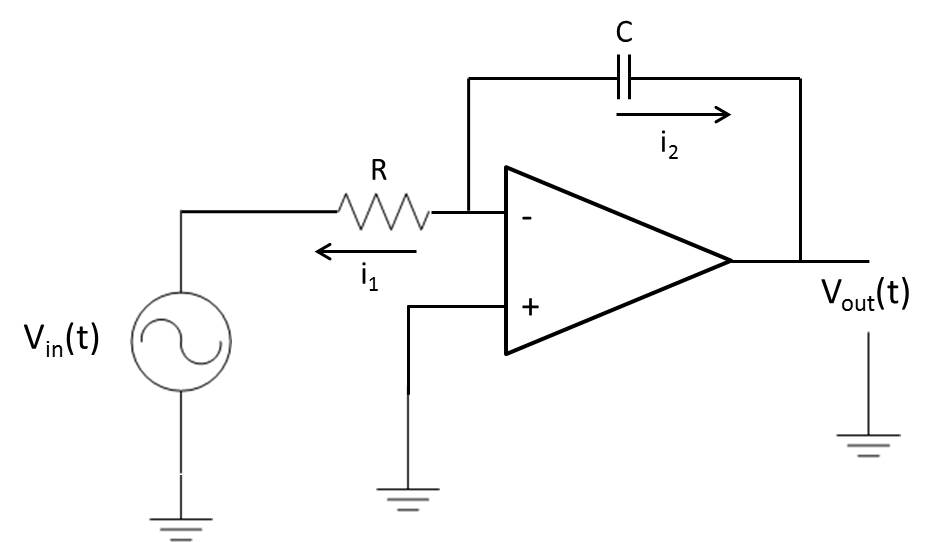
\includegraphics[width=0.5\textwidth]{Integrator.jpg}
\caption{Integrator circuit}
\label{fig: Integrator}
\end{figure}

We can start our analysis by writing a KCL equation at the inverting node:
\soln{1.25in}{
\begin{equation}
i_1(t)+i_2(t) =0
\end{equation}
which can also be written as
\begin{equation}
-\frac{v_{in}(t)}{R}-C\frac{\partial v_{out}(t)}{\partial t} =0
\end{equation}
or
\begin{equation}
\frac{v_{in}(t)}{R}+C\frac{\partial v_{out}(t)}{\partial t} =0
\end{equation}
}

Next we solve for $v_{out}(t)$

\soln{1.25in}{
\begin{equation}
\partial v_{out}(t) =-\frac{1}{RC}v_{in}(t)\partial t
\end{equation}
now we can take the integral of both sides...
\begin{equation}
\int_0^t \partial v_{out}(t) =-\frac{1}{RC}\int_0^t v_{in}(x)\partial x
\end{equation}
where x is a dummy variable of integration

\begin{equation}
v_{out}(t) =v_{out}(0)-\frac{1}{RC}\int_0^t v_{in}(x)\partial x
\end{equation}

So this circuit integrates the input....It is an integrator!
}

\newpage
\clearpage
\pagebreak

What about the circuit shown in Figure \ref{fig: Differentiator}?

\begin{figure} [h!]
\centering
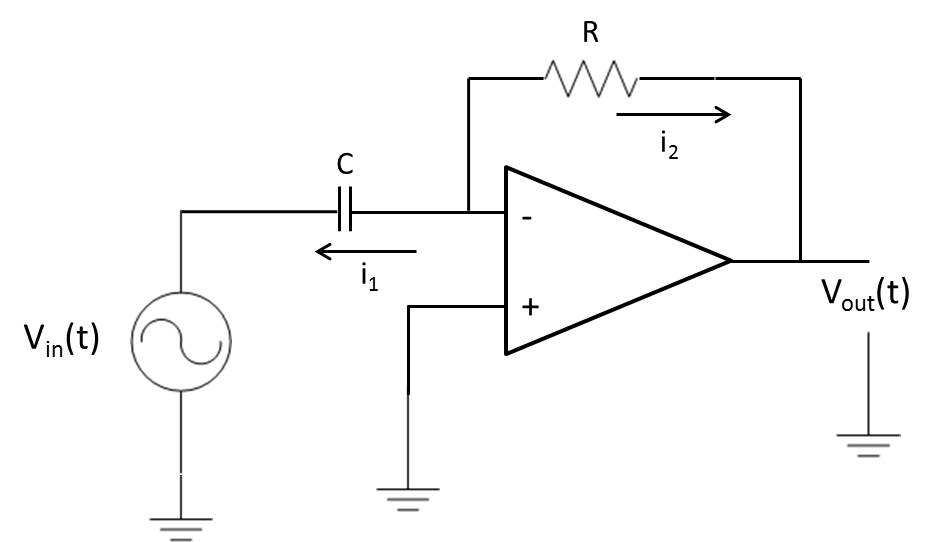
\includegraphics[width=0.5\textwidth]{Differentiator.jpg}
\caption{Differentiator circuit}
\label{fig: Differentiator}
\end{figure}

We start the analysis the same way; KCL at the inverting node
\soln{1.25in}{
\begin{equation}
i_1(t)+i_2(t) =0
\end{equation}
which can also be written as
\begin{equation}
-C\frac{\partial v_{in}(t)}{\partial t}-\frac{v_{out}(t)}{R} =0
\end{equation}
or
\begin{equation}
C\frac{\partial v_{in}(t)}{\partial t}+\frac{v_{out}(t)}{R} =0
\end{equation}
}

Next we solve for $v_{out}(t)$

\soln{1.25in}{
\begin{equation}
v_{out}(t) =-RC\frac{\partial v_{in}(t)}{\partial t}
\end{equation}


SO THIS CIRCUIT IS A DIFFERENTIATOR!!!
}

\end{document}


% Equation Array Example Code
%\begin
%{eqnarray}
%P_R &=& i_R^2R \nonumber \\
%P_R &=& (100\ mA)^2 \times 100\ \Omega \nonumber \\
%P_R &=& (100 \times 10^{-3}\ A)^2 \times 100\ \Omega \\
%P_R &=& 10000 \times 10^{-6}\ A^2  \times 100\ \Omega \nonumber \\
%P_R &=& 1\ W  \nonumber
%\end{eqnarray} 

% Figure Example Code
%\begin{figure} [h!]
%\centering
%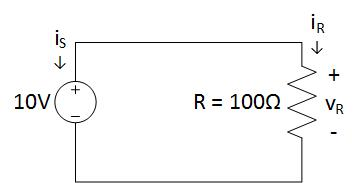
\includegraphics[width=0.5\textwidth]{OhmsLawExampleSolution.jpg}
%\caption{Ohm's Law example circuit}
%\label{fig: OhmsLawExampleSolution}
%\end{figure}

%Table Example Code
%\begin{table}[h]
%\centering
%\begin{tabular}{|l|c|c|}
%\hline
%Prefix & Abbreviation & Value \\
%\hline \hline
%Giga & $G$ & $10^9$ \\
%Mega & $M$ & $10^6$ \\
%Kilo & $k$ & $10^3$ \\
%\hline
%milli & $m$ & $10^{-3}$ \\
%micro & $\mu$ & $10^{-6}$ \\
%nano & $n$ & $10^{-9}$ \\
%pico & $p$ & $10^{-12}$ \\
%\hline
%\end{tabular}
%\caption{Engineering prefixes and values}
%\label{tab: Eng Prefixes}
%\end{table}
